% !TeX spellcheck = sk_SK
\chapter{Ako citovať}

Bibliografické informácie pre LaTeX sa ukladajú vo zvláštnom formáte BibTeX -- v súboroch s príponou \texttt{.bib}. Ukážku BibTeX záznamu pre knihu \enquote{Genetické algoritmy a genetické programování} vidno v \listingname~\ref{lst:hynek_bib}.

\begin{inlinecode}[label={lst:hynek_bib},caption={Ukážka BibTeX záznamu.},breaklines]{text}
@Book{Hynek2008,
  Title                    = {Genetické algoritmy a genetické programování},
  Author                   = {Josef Hynek},
  Publisher                = {Grada Publishing, a.s.},
  Year                     = {2008},
  Address                  = {Praha},
  ISBN                     = {978-80-7300-218-3}
}
\end{inlinecode}

\section{Príkaz \texttt{cite}}

Keď už ku danej publikácii existuje záznam, citovať ho je veľmi jednoduché -- stačí jeho identifikátor (v tomto prípade \texttt{Hynek2008}) obaliť do makra \texttt{cite}, t.j. \texttt{{\textbackslash}cite\{Hynek2008\}}. Výsledkom je citácia, ktorá sa môže podobať nasledujúcej: \cite{Hynek2008}.

Všimnite si, že citácia je \textbf{vždy súčasťou vety} -- píše sa ešte \textbf{pred bodkou}. V niektorých citačných štýloch sa citácie uvádzajú aj mimo vety/odseku, ale v našom odbore to nie je zvykom.

Do toho istého makra \texttt{cite} sa dá zapísať aj viacero identifikátorov oddelených čiarkami, napr. \texttt{{\textbackslash}cite\{Hynek2008,jabref\}}. V tom prípade vznikne hromadná citácia viacerých zdrojov: \cite{Hynek2008,jabref}.

Citácie sa dajú naopak realizovať aj podrobnejšie. Ak je napríklad žiaduce citovať konkrétnu kapitolu alebo stranu z diela, dá sa na to použiť nepovinný parameter príkazu \texttt{cite}, napr. \texttt{{\textbackslash}cite[s. 125]\{Hynek2008\}}. Výsledná citácia bude vyzerať takto: \cite[s. 125]{Hynek2008}. Takéto podrobné citácie sa však v našej odbornej oblasti prakticky vôbec nepoužívajú -- v drvivej väčšine prípadov je úplne postačujúce citovať pôvodné dielo ako celok.

\section{Parafrázy a doslovné citácie}

Doslovné citácie sa v našom odbore používajú pomerne zriedkavo. Keď hovoríme o citáciách, typicky máme na mysli nie doslovné citácie, ale parafrázy. V prípade parafráz autor práce píše text vlastnými slovami a citácie uvádza len ako zdroj, odkiaľ čerpá informácie.

Ak autor cituje doslova -- t.j. preberá konkrétne znenie textu z pôvodného zdroja -- musí citáciu viditeľne oddeliť od ostatného textu. Pri kratších úsekoch textu sa citácia označí úvodzovkami, napr.: \enquote{Genetické algoritmy sa často využívajú na riešenie rozmanitých optimalizačných úloh...} \cite{Hynek2008}.

Ak sa doslovne preberá dlhší úsek textu, napr. celý odsek alebo niekoľko odsekov, používajú sa blokové citácie, napr. \cite{Hynek2008}:
\begin{quotation}
Genetické algoritmy sa často využívajú na riešenie rozmanitých optimalizačných úloh, ale hádam ešte častejšie sa jednoduché extremálne úlohy využívajú na názorné predvedenie ich ľahkej aplikovateľnosti a funkčnosti. Aj konkrétny problém, na ktorý bude aplikovaný genetický algoritmus v tejto kapitole, je ľahko riešiteľný pomocou štandardných nástrojov matematickej analýzy, k použitiu genetického algoritmu v tejto súvislosti dochádza čisto z ilustratívnych dôvodov.
\end{quotation}
V LaTeX-u sa pre blokové citácie dá použiť napríklad prostedie \texttt{quotation}.

\subsection{Doslovné citácie v preklade}

Pravidlá pre doslovné citácie platia aj ak autor doslovne citovaný text prekladá do iného jazyka. Taký text musí byť znovu jasne oddelený od autorského textu, aj keď ho autor preložil z pôvodného jazyka. V takýchto prípadoch môže byť okrem toho užitočné uviesť (v zátvorke alebo v poznámke pod čiarou) aj pôvodné znenie textu -- to však nie je nevyhnutná podmienka.

\section{Dlhšie parafrázovanie}

Vo všeobecnosti sa je lepšie vyhnúť preberaniu dlhších častí textu -- či už formou doslovnej citácie alebo parafrázy. Autor by si mal preštudovať viacero zdrojov a spracovať svoj vlastný pohľad na problematiku.

V niektorých prípadoch sa však autor nevyhnutne musí aj v dlhšej časti textu pomerne úzko pridržiavať jedného zdroja -- napr. ak ide o normu, štandard programovacieho jazyka a pod. Keby sa na daný zdroj odvolával zakaždým, keď odtiaľ preberá informáciu, opakovala by sa tá istá citácia neprimerane často -- napríklad aj niekoľkokrát v tom istom odseku. V tom prípade môže byť dobré na začiatok podkapitoly umiestniť krátku poznámku o tom, že v nej obsiahnuté informácie alebo štruktúra textu sa čerpá z daného zdroja.

Zdôraznime, že hovoríme o autorskom texte, ktorý preberá z určitého zdroja štruktúru alebo informácie. V žiadnom prípade nesmie ísť o doslovné prebratie pôvodného textu ako takého. Doslovne prebrané state musia byť vždy citované a viditeľne oddelené od zvyšku textu, ako sme to vysvetlili vyššie.

V prípade, že sa z toho istého zdroja cituje viacero odrážok, stačí dať citáciu tesne pred odrážky a bude sa jej rozumieť tak, že platí pre všetky z nich. Ako príklad: Termín evolučné algoritmy zastrešuje predovšetkým nasledujúce techniky \cite{Hynek2008}:
\begin{itemize}
\item genetické algoritmy,
\item genetické programovanie,
\item evolučné stratégie,
\item evolučné programovanie.
\end{itemize}

\section{Príklady BibTex položiek}

V tejto časti uvedieme príklady BibTex položiek pre najčastejšie citované typy zdrojov ako sú knižné publikácie, články, elektronické zdroje a pod.

\subsection{Knižná publikácia}

BibTex položka pre knižnú publikáciu môže vyzerať napríklad nasledovne:
\begin{inlinecode}[label={lst:book_bib},caption={Ukážka BibTeX záznamu pre knihy.},breaklines]{text}
@Book{Kikimor2008,
  Title                    = {Mrkva, zemiaky a iná koreňová zelenina},
  Author                   = {Jozef Kikimor and Juraj Holota},
  Editor                   = {Jakub Hľuza},
  ISBN                     = {978-80-7252-225-1},
  Publisher                = {Grada Publishing, a.s.},
  Year                     = {2008},
  Pagetotal                = {214},  

  Address                  = {Žilina},
  Edition                  = {2. vydanie},
  Series                   = {Pokročilé témy v informatike},

  Commentator              = {Mária Čanecká},
  Subtitle                 = {Štúdie v okopávaní},
  Translator               = {Dušan Závada}
}
\end{inlinecode}

V zozname použitej literatúry sa položka zobrazí takto:

\noindent[X] \fullcite{Kikimor2008}

Počet strán je nepovinná informácia -- v našom odbore je konvenciou ju skôr vynechať. Kniha nemusí mať podtitul, meno komentátora, prekladateľa, označenie vydania a série a podobne -- v tom prípade sa samozrejme takisto nezadávajú.

\subsubsection{Viac než traja autori}

Ak má publikácia viac než troch autorov, v citácii sa zobrazí len meno prvého autora a skratka \enquote{et al.}. Do poľa \texttt{author} treba zapísať mená všetkých autorov a nechať LaTeX, aby sám vygeneroval citáciu v požadovanom formáte, napr.:
\begin{inlinecode}[breaklines]{text}
@Book{Koropnik2005,
  Title                    = {Zemiakové delo a iné nástroje},
  Author                   = {Ondrej Koropník and Justín Ďuroška and Albín Chovanec and Filip Hurta},
  ISBN                     = {978-80-7332-225-2},
  Publisher                = {Hľuza Publishing},
  Year                     = {2005},

  Address                  = {Lopušné pažite}
}  
}
\end{inlinecode}
Citácia má štyroch autorov, preto LaTeX automaticky zoberie do úvahy len meno prvého autora a zvyšok nahradí skratkou \enquote{et al.} (z lat. et alii -- a kolektív):

\noindent[X] \fullcite{Koropnik2005}

\subsubsection{Chýbajúce ISBN}

ISBN číslo je povinná položka. Niektoré staršie vydania kníh nemusia mať ISBN číslo -- t.j. mohli byť vydané ešte pred zavedením ISBN. V tom prípade sa pochopiteľne neuvádza, napr.:

\noindent[X] \fullcite{Urbanova1980}

\subsubsection{Publikácie s neznámym autorom}

Niektoré knižné publikácie nemusia mať uvedeného autora, platí to napr. pri niektorých druhoch oficiálnych dokumentov \cite{boldis1}:

\noindent[X] \fullcite{crzp}

\subsubsection{Autorom je korporácia}

Alebo môže byť autorom nejaká korporácia -- v tom prípade sa jej názov uvádza, ak nie je totožný s názvom vydavateľstva, inak sa nemusí uviesť \cite{boldis1}.

\subsubsection{Stať z knihy}

Ak z knihy citujeme len nejakú časť -- napr. určitý rozsah strán -- môže sa táto informácia tiež uviesť. Použije sa na to pole \texttt{pages}, napr. \texttt{pages = \{112{-}{-}125\}}. Výsledok sa zobrazí nasledovne:

\noindent[X] \fullcite{Kikimor2008Pages}

\subsection{Kapitola v knihe}

Ak sa z knihy cituje jedna konkrétna kapitola, dá sa použiť záznam typu \texttt{inbook} a špecifikovať číslo kapitoly (príp. aj jej názov) v poli \texttt{chapter}, napr.:
\begin{inlinecode}[breaklines]{text}
@InBook{Kikimor2008IB,
  Title                    = {Mrkva, zemiaky a iná koreňová zelenina},
  
  [...]
  
  Chapter                  = {5},
  
  [...]
  
}
\end{inlinecode}

Výsledný záznam sa zobrazí nasledovne:

\noindent[X] \fullcite{Kikimor2008IB}

Ak ide o knihu, kde každá kapitola má iného autora (príp. autorov), cituje sa kapitola rovnako ako príspevok v zborníku -- viď časť \ref{sec:inproc}.

\subsection{Príspevok v zborníku}
\label{sec:inproc}

Na citovanie príspevkov v zborníkoch môžeme použiť záznam typu \texttt{incollection}, napr.:
\begin{inlinecode}[breaklines]{text}
@Incollection{floreanoEpuck,
  Title                    = {E-puck: A Robotic Platform for Studying the Evolution of Communication},
  Author                   = {Floreano, Dario and Mitri, Sara and Hubert, Julien},
  Booktitle                = {Evolution of Communication and Language in Embodied Agents},
  ISBN                     = {978-3-642-01250-1},
  Publisher                = {Springer},
  Year                     = {2009},
  Editor                   = {Stefano Nolfi and Marco Mirolli}
}
\end{inlinecode}

Ako vidno, názov (príp. podnázov) knihy sa píše do poľa \texttt{booktitle} (resp. \texttt{booksubtitle}). Do poľa \texttt{title} sa teraz píše názov citovaného príspevku. Výsledný záznam sa zobrazí nasledovne:

\noindent[X] \fullcite{floreanoEpuck}

Ak nejde o zborník v pravom zmysle slova, ale o knižnú publikáciu, kde každá kapitola má iných autorov, je možné navyše zadať aj číslo kapitoly v poli \texttt{chapter}.

\subsection{Článok v časopise}

Na citovanie článku v časopise je možné použiť záznam typu \texttt{article}. Pri časopisových článkoch sa povinne uvádza ISSN. Ak sú k dispozícii, treba uviesť aj informácie o zväzku (\angl{volume}) a čísle (\angl{number}). Záznam môže vyzerať napríklad takto:
\begin{inlinecode}[breaklines]{text}
@Article{Bhasin2011,
  Title                    = {Asymptotic tracking by a reinforcement learning-based adaptive critic controller},
  Author                   = {Bhasin, Shubhendu and Sharma, Nitin and Patre, Parag and Dixon, Warren},
  Journal                  = {Journal of Control Theory and Applications},
  Year                     = {2011},

  ISSN                     = {0974-5572},
  Number                   = {3},
  Pages                    = {400--409},
  Publisher                = {Springer},
  Volume                   = {9}
}
\end{inlinecode}
a výsledná citácia nasledovne:

\noindent[X] \fullcite{Bhasin2011}

\subsection{Časopis ako celok}

Vo vzácnych prípadoch sa dá citovať aj časopis ako celok -- možno na to použiť záznam typu \texttt{periodical}, napr.:
\begin{inlinecode}[breaklines]{text}
@Periodical{periodical2014,
  Title                    = {Časopis nových vynálezov},
  Year                     = {2014},
  ISSN                     = {1211-0748},
  Number                   = {12},
  Volume                   = {4},

  Address                  = {Čabracký Vrbovok},
  Publisher                = {Hľuza Publishing},
  Timestamp                = {2017.09.18}
}
\end{inlinecode}
Výsledná citácia bude vyzerať nasledovne:

\noindent[X] \fullcite{periodical2014}

\subsection{Elektronický zdroj}

V prípade elektronických zdrojov môžeme použiť záznam typu \texttt{electronic}. Povinná je položka \texttt{howpublished}, ktorá bližšie špecifikuje typ elektronického zdroja. U nás to bude najčastejšie \enquote{online}, ale môže byť napr. aj \enquote{CD-ROM} a pod. Pre \enquote{online} záznamy je povinné uviesť URL a dátum, kedy bol príslušný zdroj citovaný (v poli \texttt{urldate}). Ako príklad môžeme uviesť:
\begin{inlinecode}[breaklines]{text}
@Electronic{latexTables,
  Title                    = {LaTeX/Tables},
  HowPublished             = {online},
  Url                      = {https://en.wikibooks.org/wiki/LaTeX/Tables},
  Urldate                  = {2017-08-22}
}
\end{inlinecode}

Výsledné citácie môžu vyzerať napríklad nasledovne:

\noindent[X] \fullcite{jabref}

\noindent[X] \fullcite{latexFigures}

\section{Nástroj JabRef}

BibTeX záznamy prirodzene nie je nutné zapisovať ručne priamo v kóde -- existujú na to pomocné nástroje. Jedným z nich je napríklad aplikácia JabRef \cite{jabref}, ktorá poskytuje užitočné grafické rozhranie na editáciu BibTeX súborov. Ukážka rozhrania je na \figurename~\ref{fig:jabref}.

\begin{figure}
\centering
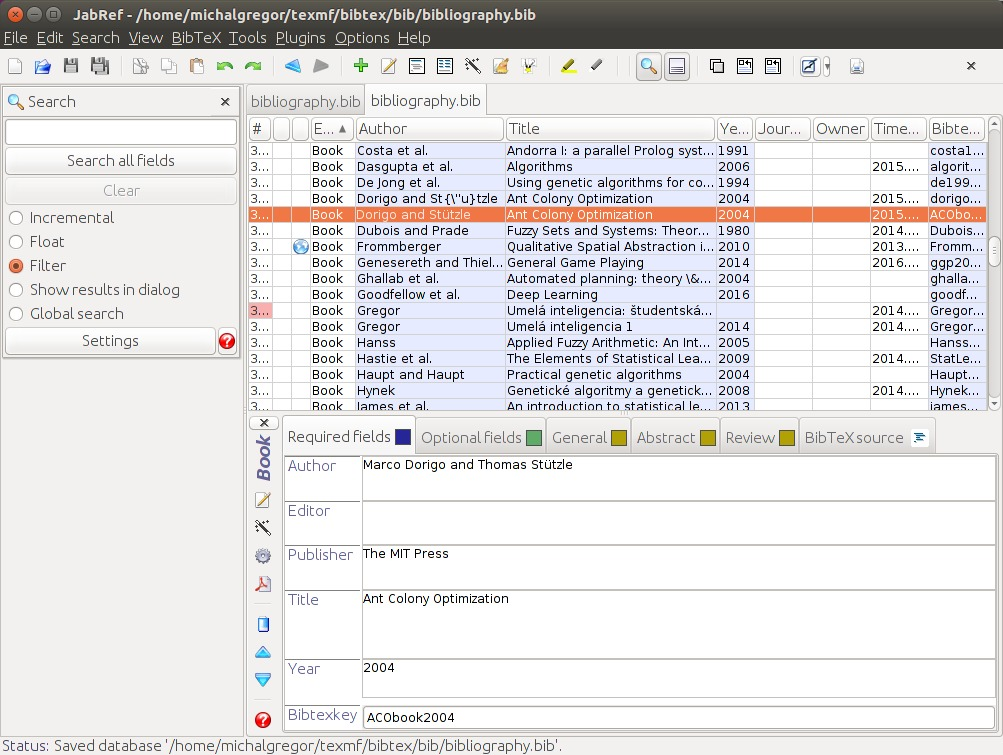
\includegraphics[width=14cm]{jabref}
\caption{Grafické rozhranie aplikácie JabRef.}
\label{fig:jabref}
\end{figure}
